\begin{subsectionframemod}{Difference between Natural and Aerial Images}
    La plupart des méthodes sont évaluées sur des images naturelles : les ensembles de données Pascal VOC et MS COCO.
    $\Rightarrow$ cela ne garantit pas de bonnes performances sur les images aériennes.
    \vspace{2mm}


    Les tailles des objets sont extrêmement différentes entre les images aériennes et naturelles.

    \begin{figure}
        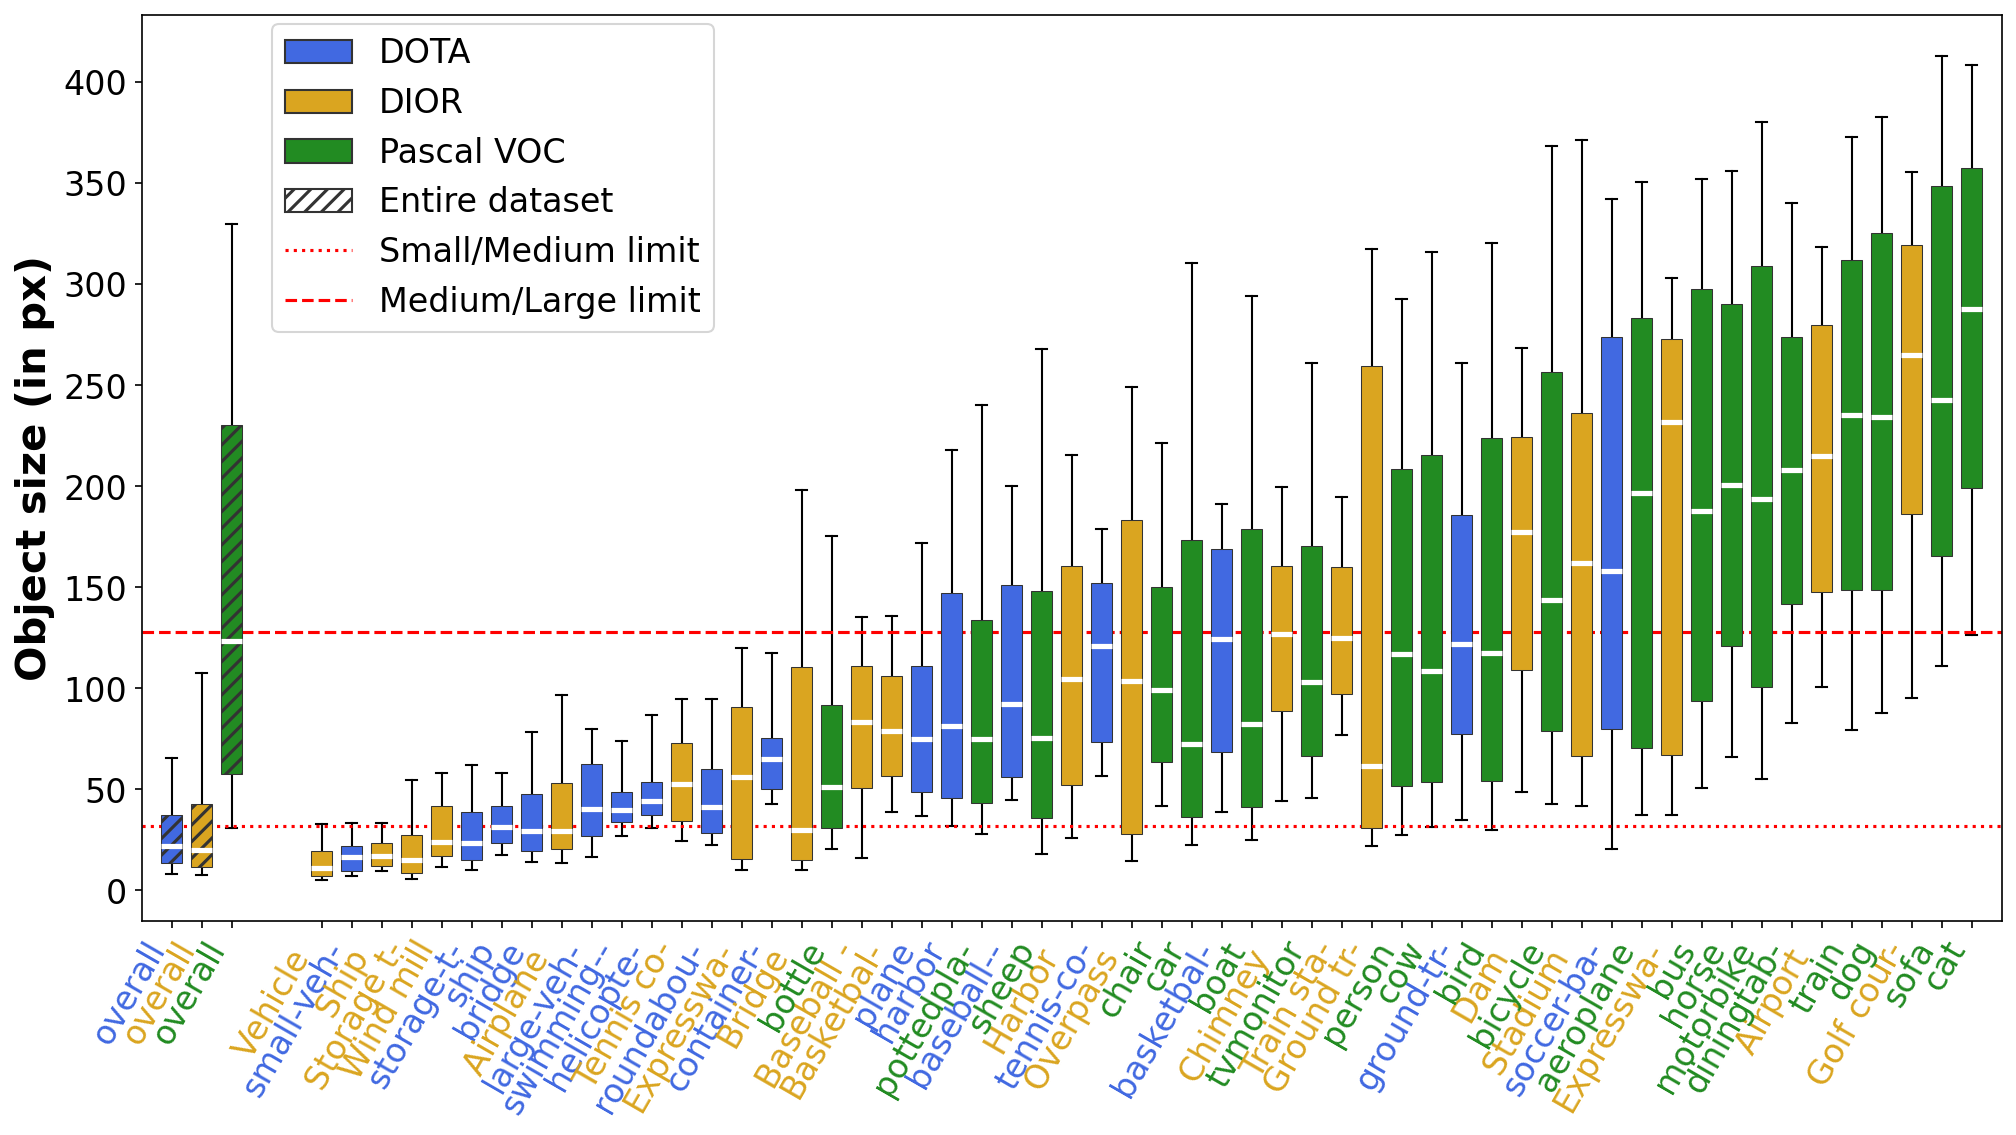
\includegraphics[width=0.8\textwidth]{Figures/object_sizes.png}
    \caption{Diagramme en boîte des tailles d'objets dans DOTA (\cite{xia2018dota}), DIOR (\cite{li2020object}) et Pascal VOC (\cite{everingham2010pascal}); par classe \textbf{(à droite)} et globalement \textbf{(à gauche)}.}
    \end{figure}

    

    
\end{subsectionframemod}